\documentclass[12pt,a4paper,english]{extarticle}
\usepackage[T1]{fontenc}
\usepackage[utf8]{inputenc}
\usepackage{fourier}
\usepackage{geometry}
\geometry{verbose,tmargin=2.5cm,bmargin=2cm,lmargin=2.5cm,rmargin=2cm}
\usepackage{float}
\usepackage{textcomp}
\usepackage{amsmath}
\usepackage{stackrel}
\usepackage{graphicx}
\usepackage{esint}
\usepackage{tikz}
\usetikzlibrary{matrix,calc}

\makeatletter

\providecommand{\tabularnewline}{\\}

\usepackage{fancyhdr}
\usepackage{lscape}
\usepackage{amssymb}
\pagestyle{fancy}
\lhead{Electronica III - 22.13}
\chead{TPL1}
\rhead{ITBA}
\renewcommand{\headrulewidth}{1pt}
\renewcommand{\footrulewidth}{1pt}

\makeatother

\usepackage[english]{babel}
\input{setup/BaseKarnaugh.tex}

\usepackage{listings}
\newcommand{\horrule}[1]{\rule{\linewidth}{#1}}

\title{
        %\vspace{-1in} 	
        \usefont{OT1}{bch}{b}{n}
        \normalfont \normalsize \textsc{Instituto Tecnológico de Buenos Aires} \\ [25pt]
        \horrule{0.5pt} \\[0.4cm]
        \huge Trabajo Práctico de Laboratorio Nro. 1 \\
        \horrule{2pt} \\[0.5cm]
}
\author{
        \normalfont 								\normalsize
        NOWIK, Ariel 58309\\[-3pt]		\normalsize
        MASPERO, Martina 57120\\[-3pt]		\normalsize
        MESTANZA, Joaquin 58288\\[-3pt]		\normalsize
        REGUEIRA, Marcelo 58300\\[-3pt]		\normalsize
        \today
}
\date{}



%%% Begin document
\begin{document}
% The \input command appends the content of the file directly into the document.
\maketitle
\newpage

\section*{Task 1}

The program is called this way 'run a b c'

The parameters are:
\begin{itemize}
  \item $a$: tells whether the input is unsigned or signed (0/1)
  \item $b$: size (in bits) of the integer part of the number ($\geq0$)
  \item $c$: size (in bits) of the decimal part of the number ($\geq0$)
\end{itemize}
All inputs should be numbers. Also b and c can't be 0 at the same time.
All these things are validated.

The program logic uses simple formulas to solve the problem separately in signed and unsgined case.
The inituition beyond the formulas was obtained by looking at the composition of binary number.
\begin{figure}[H]
  \begin{centering}
  \includegraphics[scale=1]{data/bits.png}
  \par\end{centering}
  \caption{View of the value of each bit}
\end{figure}
As lowest significant bit worths $2^{-c}$ then the resolution is $2^{-c}$ and this works in both signed and unsigned cases
\\
Thought, to compute the range we need to separate in two cases, looking at which are the greatest (we call it $r$) and lower (we call it $l$) numbers we can make in each case
In the unsgined case the lower number is 0 and the highest will be
$$r=\underbrace{2^{-c}+2^{-c+1}+...+2^{-1}}_{1-2^{-c}}+\underbrace{1+2^{1}+...+2^{b-1}}_{2^{b}-1}=2^{b}-2^{-c}$$
So the resolution is just $r-l=2^{b}-2^{-c}$
\\
With the signed case we note the smallest number is when only most significant bit is 1
$$l=-2^{b-1} $$
And the highest when all bits are 1 except the most significant one
$$r=2^{-c}+2^{-c+1}+...+2^{1}+1+2^{1}+...+2^{b-2}=2^{b-1}-2^{-c}$$
Thus the resolution is $r-l=2^{b-1}-2^{-c}+2^{b-1}=2^{b}-2^{-c}$
That is the same, that is reasonable because we can express the same amount of numbers with the same amount of bits and that doesn't depend on whether the number is signed or not



\section*{Task 2}

Starting with the following function expressed in maxterms:
\[
    f(d,c,b,a)=\prod{(M_{0},M_{1},M_{5},M_{7},M_{8},M_{10},M_{14},M_{15})}
\]

Taking $d,c,b,a$ as input variables. For simplify, the same 
function is expressed in minterms to operate later:
\[
    f(d,c,b,a)=\sum{(m_{2},m_{3},m_{4},m_{6},m_{9},m_{11},m_{12},m_{13})}
\]

Starting with it, we build the function without simplifying:
\[
    f(d,c,b,a)=(\overline{d} \cdot \overline{c} \cdot b \cdot \overline{a})+
    (\overline{d} \cdot \overline{c} \cdot b \cdot a)+
    (\overline{d} \cdot c \cdot \overline{b} \cdot \overline{a})+
    (\overline{d} \cdot c \cdot b \cdot \overline{a})+
    (d \cdot \overline{c} \cdot \overline{b} \cdot a)+
    (d \cdot \overline{c} \cdot b \cdot a)+
    (d \cdot c \cdot \overline{b} \cdot \overline{a})+
    (d \cdot c \cdot \overline{b} \cdot a)
\]

We grouped by common factor in a convenient way:
\begin{eqnarray}
    \nonumber f(d,c,b,a)&=&\underbrace{(\overline{d} \cdot \overline{c} \cdot b \cdot \overline{a})+
    (\overline{d} \cdot \overline{c} \cdot b \cdot a)}+\underbrace{
    (\overline{d} \cdot c \cdot \overline{b} \cdot \overline{a})+
    (\overline{d} \cdot c \cdot b \cdot \overline{a})}+\underbrace{
    (d \cdot \overline{c} \cdot \overline{b} \cdot a)+
    (d \cdot \overline{c} \cdot b \cdot a)}+\\
    \nonumber &\longrightarrow&\underbrace{(d \cdot c \cdot \overline{b} \cdot \overline{a})+
    (d \cdot c \cdot \overline{b} \cdot a)}
\end{eqnarray}
\[
    f(d,c,b,a)=[\overline{d} \cdot \overline{c} \cdot b \cdot \underbrace{(\overline{a}+a)}_1]+
    [\overline{d} \cdot c \cdot \overline{a} \cdot \underbrace{\overline{b}+b)}_1]+
    [d \cdot \overline{c} \cdot a \cdot  \underbrace{(\overline{b}+b)}_1]+
    [d \cdot c \cdot \overline{b} \cdot \underbrace{(\overline{a}+a)}_1]
\]
\[
    \boxed{f(d,c,b,a)=(\overline{d} \cdot \overline{c} \cdot b)+
    (\overline{d} \cdot c \cdot \overline{a})+
    (d \cdot c \cdot \overline{b})+
    (d \cdot \overline{c} \cdot a)}
\]
\\ %Salto de linea
Analogously, starting with the expresssion in minterms we reduce 
the function through a map of Karnaugh:

\begin{centering}
    \begin{Karnaugh}
        \minterms{2,3,4,6,9,11,12,13}
        \maxterms{0,1,5,7,8,10,14,15}
        \implicant{3}{2}{red}
        \implicantcostats{4}{6}{red}
        \implicant{12}{13}{red}
        \implicant{9}{11}{red}
    \end{Karnaugh}
\par\end{centering}

From the first group (first row) we have that $d$, $c$ and $b$ 
are constantes, thus the first factor stays the way 
$ \overline{d} \overline{c} b$.\par
From the second group (second row) we have $d$, $c$ and $a$ as
constants, thus this factor stays as $ \overline{d} c \overline{a}$.\par
From the third group (third row) remain constant $d$, $c$ and $b$, thus 
this factor stays as $d c \overline{b}$.\par
Finally, from the last row, in the group $d$, $c$ and $a$ stay constant, 
thus this factor stays the way
$d \overline{c} a$.\par
Adding the partial termns we get the simplified function:
\[
    \boxed{f(d,c,b,a)=(\overline{d} \cdot \overline{c} \cdot b)+
    (\overline{d} \cdot c \cdot \overline{a})+
    (d \cdot c \cdot \overline{b})+
    (d \cdot \overline{c} \cdot a)}
\]
Wich is the same obtained by simplification by boolean algebra. \par
Taking this function, it was implemented in a logical circuit
 by AND, OR and NOT gates, as shown below.

\begin{figure}[H]
    \begin{centering}
    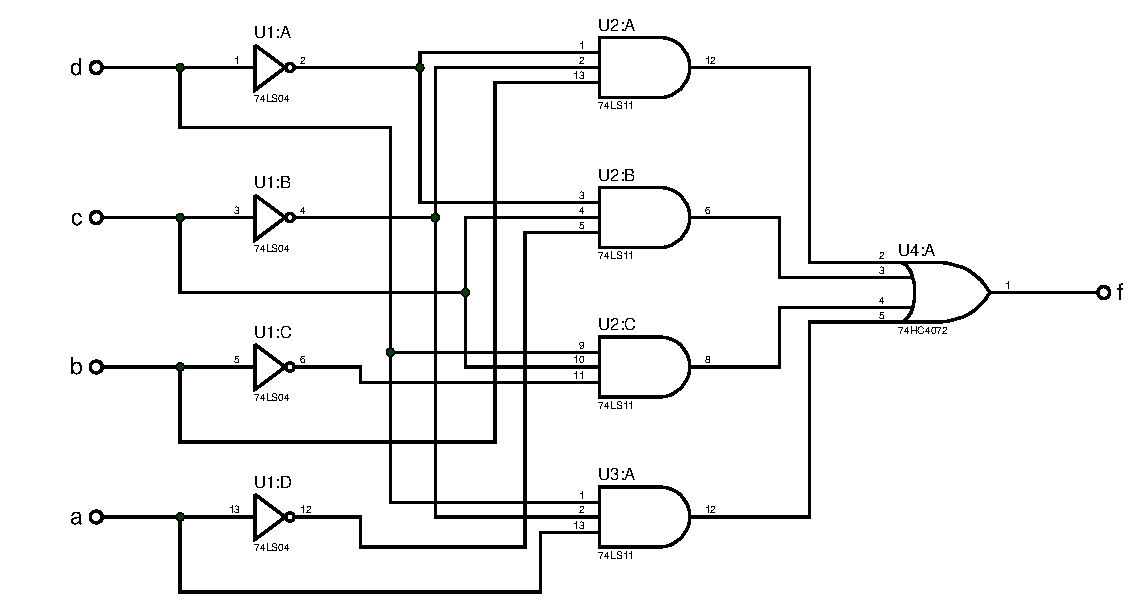
\includegraphics[width=1\textwidth]{data/ImplementacionEj2}
    \par\end{centering}
    \caption{Logical circuit that implements $f(d,c,b,a)$ - Made in Proteus 7.8}
\end{figure}

For implementation using only NOR gates, first we have to work
 with the obtained function applyin boolean algebra properties. 
 Taking the function:
\[
    f(d,c,b,a)=(\overline{d} \cdot \overline{c} \cdot b)+
    (\overline{d} \cdot c \cdot \overline{a})+
    (d \cdot c \cdot \overline{b})+
    (d \cdot \overline{c} \cdot a)
\]
\par
We twice denied the terms separated by sums, for keeping the equal:
\[
    f(d,c,b,a)=\overline{\overline{(\overline{d} \cdot \overline{c} \cdot b)}}+
    \overline{\overline{(\overline{d} \cdot c \cdot \overline{a})}}+
    \overline{\overline{(d \cdot c \cdot \overline{b})}}+
    \overline{\overline{(d \cdot \overline{c} \cdot a)  }}
\]
\par
Next we deny the factors only once, for turning the products 
into sums (property of De Moivre):
\[
    \boxed{f(d,c,b,a)=\overline{(d+c+\overline{b})}+
    \overline{(d+\overline{c}+a)}+
    \overline{(\overline{d}+\overline{c}+b)}+
    \overline{(\overline{d}+c+\overline{a})}}
\]
\par

Having the expression in terms of sums, it is possible to implement 
the circuit using only NOR gates, as shown below.

\begin{figure}[H]
    \begin{centering}
    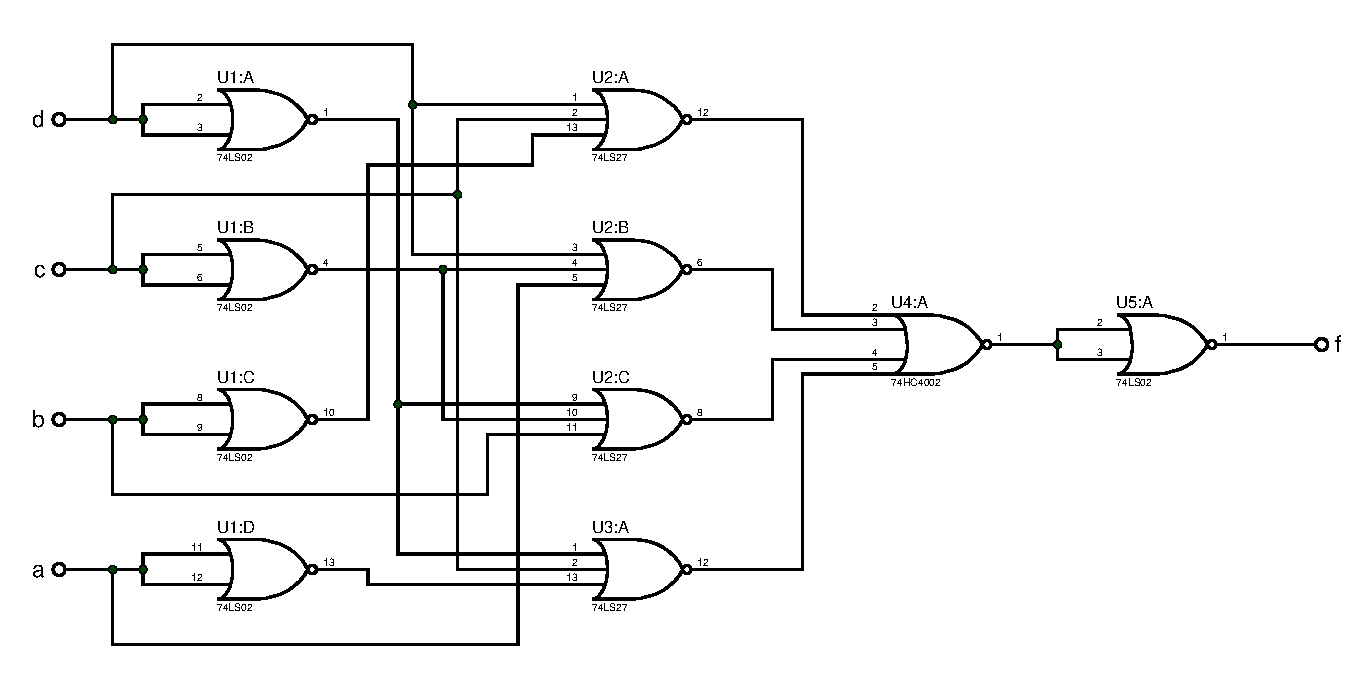
\includegraphics[width=1\textwidth]{data/ImplementacionEj2_NOR}
    \par\end{centering}
    \caption{Logical circuit that implements $f(d,c,b,a)$
    with NOR gates - Made in Proteus 7.8}
\end{figure}





\section*{Task 3}

\subsection*{Decoder}

\begin{figure}[H]
  \begin{centering}
  \includegraphics[scale=1]{data/decoder.png}
  \par\end{centering}
  \caption{Block Diagram of a $N:2^{N}$ Decoder}
\end{figure}


The binary decoder is a combinational logic device with N input lines and $2^{n}$ output lines, one particular combination of inputs activates one output while the remaining ones are disabled. The decoder only works when the enable input is on. Below you can find the truth table of a 2 input decoder:

\begin{figure}[H]
  \begin{centering}
  \includegraphics[scale=1]{data/decodertable.png}
  \par\end{centering}
  \caption{Truth table of a 2:4 Decoder}
\end{figure}


\begin{figure}[H]
  \begin{centering}
  \includegraphics[scale=1]{data/decoderlogic.png}
  \par\end{centering}
  \caption{Logic Implementation of a 2:4 Decoder}
\end{figure}


\subsection*{Multiplexer}

\begin{figure}[H]
  \begin{centering}
  \includegraphics[scale=1]{data/muxB.png}
  \par\end{centering}
  \caption{Block Diagram of a $2^{M}:1$ Multiplexer}
\end{figure}

A multiplexer, also known as 'mux', is another combinational circuit that has $2^{M}$ inputs, M select lines and one single output. The select input lines control which data input is connected to the output. The function of a 2 input Mux is described by the truth table shown below:


\begin{figure}[H]
  \begin{centering}
  \includegraphics[scale=1]{data/muxtable.png}
  \par\end{centering}
  \caption{Truth table of a 2:1 Mux}
\end{figure}


\subsection*{About the code}

In one hand, both mux.v and decoder.v, use conditional statements to describe their behavior. This way is easier for the user to understand how the devices work.
Each module has it's own test bench which considers all possible inputs for a complete test.

On the other hand, newmux.v and newdecoder.v, have a variable parameter which changes the number of inputs the devices could have. The way that they are implemented is more difficult to understand than the behavioral modeling, but it is shorter. For the decoder, the shift operator resumes perfectly its function and for the mux, the index of the input array chooses the element that has to be in the output.
In order to simplify the code, instead of N input/output lines of 1 bit, it has an array of all the input's bits together. 
  



\section*{Task 4}
    In this case we need to convert a 4-bit number into its complement 
    to two. A truth table is built first with four outputs corresponding 
    to the four input bits of the number complemented, as shown below.
    \begin{table}[H]
        \begin{center}
        \begin{tabular}{|c|c|c|c||c|c|c|c|}
        \hline
        \multicolumn{4}{|c||}{4-Bit In} & \multicolumn{4}{|c|}{2-Comp. Out}
        \\ \hline
        $d$ & $c$ & $b$ & $a$ & $f_{d}$ & $f_{c}$ & $f_{b}$ & $f_{a}$\\
        \hline \hline
        0 & 0 & 0 & 0 & 0 & 0 & 0 & 0\\ \hline
        0 & 0 & 0 & 1 & 1 & 1 & 1 & 1\\ \hline
        0 & 0 & 1 & 0 & 1 & 1 & 1 & 0\\ \hline
        0 & 0 & 1 & 1 & 1 & 1 & 0 & 1\\ \hline
        0 & 1 & 0 & 0 & 1 & 1 & 0 & 0\\ \hline
        0 & 1 & 0 & 1 & 1 & 0 & 1 & 1\\ \hline
        0 & 1 & 1 & 0 & 1 & 0 & 1 & 0\\ \hline
        0 & 1 & 1 & 1 & 1 & 0 & 0 & 1\\ \hline
        1 & 0 & 0 & 0 & 1 & 0 & 0 & 0\\ \hline
        1 & 0 & 0 & 1 & 0 & 1 & 1 & 1\\ \hline
        1 & 0 & 1 & 0 & 0 & 1 & 1 & 0\\ \hline
        1 & 0 & 1 & 1 & 0 & 1 & 0 & 1\\ \hline
        1 & 1 & 0 & 0 & 0 & 1 & 0 & 0\\ \hline
        1 & 1 & 0 & 1 & 0 & 0 & 1 & 1\\ \hline
        1 & 1 & 1 & 0 & 0 & 0 & 1 & 0\\ \hline
        1 & 1 & 1 & 1 & 0 & 0 & 0 & 1\\ \hline
        \end{tabular}
        \caption{Outputs with complement to two.}
        \end{center}
        \end{table}
        \par
        The output functions are expressed based on the minternms.
        They are simplified using Karnaugh's Maps. Starting with $f_d$ function:\par
        \[
            f_{d}=\sum{(m_1,m_2,m_3,m_4,m_5,m_6,m_7,m_8)}
        \]
        \begin{centering}
            \begin{Karnaugh}
                \minterms{1,2,3,4,5,6,7,8}
                \maxterms{0,9,10,11,12,13,14,15}
                \implicantsol{8}{red}
                \implicant{4}{6}{red}
                \implicant{1}{3}{red}
                \implicant{2}{6}{blue}
            \end{Karnaugh}
        \par\end{centering}
        Solving the map with the indicated groups, the simplified 
        function remains as:
        \[
            \boxed{f_{d}=(d \cdot \overline{c} \cdot \overline{b} \cdot \overline{a})+
            (\overline{d} \cdot c)+(\overline{d} \cdot \overline{c} \cdot a)+
            (\overline{d} \cdot b \cdot \overline{a})}    
        \]
     
        Now, taking the $f_c$ function, we do the same:
        \[
            f_{c}=\sum{(m_1,m_2,m_3,m_4,m_9,m_{10},m_{11},m_{12})}
        \]
        \begin{centering}
            \begin{Karnaugh}
                \minterms{1,2,3,4,9,10,11,12}
                \maxterms{0,5,6,7,8,13,14,15}
                \implicant{4}{12}{red}
                \implicantdaltbaix{2}{10}{red}
                \implicantdaltbaix{1}{11}{red}
            \end{Karnaugh}
        \par\end{centering}
        With the indicated groups, we get the simplified funcion:
        \[
            \boxed{f_c=(c \cdot \overline{b} \cdot \overline{a})+
            (\overline{c} \cdot a)+
            (\overline{c} \cdot b \cdot \overline{a})}    
        \]\par
        Next, with the $f_b$ function:
        \[
            f_{b}=\sum{(m_1,m_2,m_5,m_6,m_9,m_{10},m_{13},m_{14})}    
        \]
        \begin{centering}
            \begin{Karnaugh}
                \minterms{1,5,13,9,2,6,14,10}
                \maxterms{0,4,12,8,3,7,15,11}
                \implicant{1}{9}{red}
                \implicant{2}{10}{red}
            \end{Karnaugh}
        \par\end{centering}
        Solving the map, we get:
        \[
            \boxed{f_b=(\overline{b} \cdot a)+(b \cdot \overline{a})}    
        \]\par
        For the last function $f_a$:
        \[
            f_{a}=\sum{m_1,m_3,m_5,m_7,m_9,m_{11},m_{13},m_{15}}    
        \]\par
        In the table it can be observed that the output depends 
        directly from input $a$. We can write the simplified 
        function without making the Karnaugh's map:
        \[
            \boxed{f_a=a}    
        \]
        \par
        Having already the four output functions, the implementation
        can be carried out in a circuit with AND, OR and NOT logic gates,
        as shown in the next page.
       
        \begin{figure}[H]
            \begin{centering}
            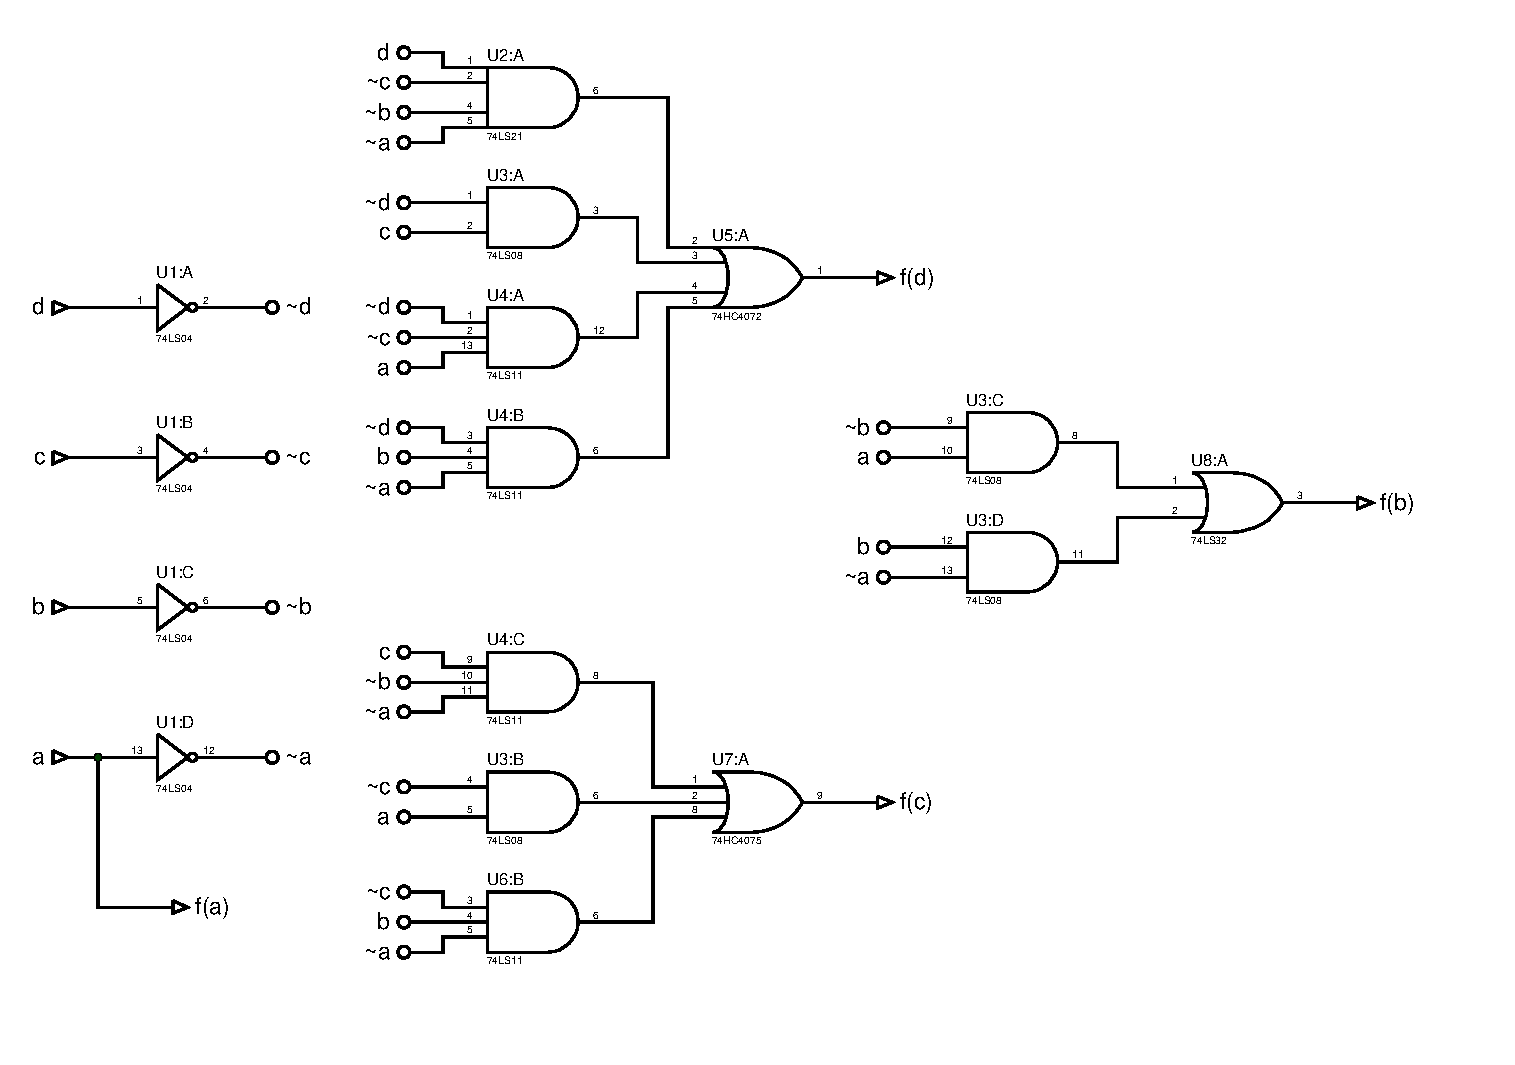
\includegraphics[width=1\textwidth]{data/ImplementacionEj4}
            \par\end{centering}
            \caption{data/Implementation of 2-complement circuit for a 4-bit input number - Designed in Proteus 7.8}
        \end{figure}
        



\section*{Task 5}

%\title{Introduction to \LaTeX{}}
%\author{Author's Name}
%\maketitle

%\begin{abstract}
%The abstract text goes here.
%\end{abstract}


\section{Two BCD addition}

\begin{figure}[H]
  \begin{centering}
  \includegraphics[scale=0.5]{data/ej5.png}
  \par\end{centering}
  \caption{Block diagram of the 4-Bit BCD sum}
\end{figure}
Given two numbers in BCD format, return the two-digits value of the sum of these two numbers.
In order to implement this task, two 4-bit Full Adders were instantiated from the same module.
Assuming that inputs are valid, there are just two cases to analyze. 
First of all, if the sum of the two numbers in decimal is greater than 9 or the carryout bit from the first Full Adder, the sum of them showed in binary code is not the actual BCD.   
To get the right answer it's necessary to add 6 in decimal value to the sum of those two numbers in order to get the BCD equivalent. Otherwise, there is not addition to the sum of those two numbers.


%\begin{equation}
%    \label{simple_equation}
%    \alpha = \sqrt{ \beta }
%\end{equation}

\subsection{Input}
Two BCD digits must be entered with the following format:
./a.out +a=XXXX +b=YYYY
Where a.out is the name of output executable and both XXXX and YYYY are two 4-bit binary numbers.
\subsection{Output}
The output number is shown as an 8-bit BCD format.

%\section{Conclusion}
%Write your conclusion here.


\section*{Task 6}

\subsection*{Module overview}
The program module dependencies are organized this way
\begin{figure}[H]
  \begin{centering}
  \includegraphics[scale=1]{data/modulos.png}
  \par\end{centering}
  \caption{Module dependencies}
\end{figure}
Each module has its own executable file to run their tests. The modules are

\begin{itemize}
  \item $Mux$: It connects the corresponding operation wire with corresponding output. It is an 8 input mux with inputs of size 4.
  \item $4\;bit\;adder$: Its function is to add 4 bit numbers and compute carry and overflow flags of that operations
  \item $Fulladder$: Adds 1 bit numbers with carry in, and carry out functionality
  \item $Adder $: Basic one bit number adder with carry functionality
\end{itemize}

Currently sum and substract are built from scratch, other operations use verilog built-in fucntions, altough, it would not cause any compatibility problem to have these functions manually coded.

Now we will analize in more depth how the program works

\subsection*{ALU overview}

\begin{figure}[H]
  \begin{centering}
  \includegraphics[scale=1]{data/alu.png}
  \par\end{centering}
  \caption{Alu in-out}
\end{figure}

The ALU makes sure the output and flags are correct accoring to opcodes and inputs.
\subsection*{Operations}
There are 8 operations
\begin{itemize}
  \item \textbf{addition} (000) : Implemented using 4 bit full adder
  \item \textbf{difference} (001): Implemented using 4 bit full adder using carry in and built-in not operator
  \item \textbf{and} (010): Implemented with built-in function
  \item \textbf{or} (011): Implemented with built-in function
  \item \textbf{not} (100): Implemented with built-in function
  \item \textbf{xor} (101): Implemented with built-in function
  \item \textbf{2'th complement} (110): Implemented with built-in function
  \item \textbf{shift left} (111): Implemented with built-in function
\end{itemize}

All 8 operations are connected into a wire array, then Mux comes into action and select according to opcode which action write to output
Also another important detail is that operations that use only one number use input 1, and ignore input 2

There are four flags
\begin{itemize}
  \item \textbf{carry/overflow} (Managed by 4 bit adder modules)
  \item \textbf{zero/negative} (Easily managed directly by ALU)
\end{itemize}
It is important to note that operations that do not use carry and overflow make these bits to be 0.

\subsection*{Mux}
\begin{figure}[H]
  \begin{centering}
  \includegraphics[scale=1]{data/mux.png}
  \par\end{centering}
  \caption{Mux in-out}
\end{figure}

This is a very simple module, implemented using vectorized expresions. It justs decides which input is wired to output according to selector input

\subsection*{Full 4bit Adder}

\begin{figure}[H]
  \begin{centering}
  \includegraphics[scale=1]{data/4bitadder.png}
  \par\end{centering}
  \caption{Full 4bit Adder in-out}
\end{figure}

This module adds two binary 4 bit number with carry-in, carry-out functionality. Also it computes the overflow flag by making the xor of the 'last bit' carry and the carry-out
Also , to function this module uses 4 single full adders connected in 	
cascade. We won't describe these modules in this file because they are standard and the sources are enough.



%%% End document
\end{document}
